\chapter{\uppercase{Impact of Output Quantities on Accuracy} \label{chapter:03}}

Here, we motivate the reduction of a quantity called \emph{skewness} in pursuit of optimizing the geometry of set-valued solutions to stochastic inverse problems with respect to their ability to be well-approximated by Monte-Carlo integration.
However, the results hold for any attempt to approximate densities defined on sets induced by random samples, and thus may be of interest to the larger research community.

We demonstrate that the number of samples required to approximate densities using uniform i.i.d.~sampling is proportional to the skewness of the map used for inversion, though the convergence rate of the algorithm used to solve the stochastic inverse problem is unaffected.


\section{Skewness and Information Content}\label{sec:skewness}
In \cite{BGE+15}, the concept of skewness in a QoI map $\qoi$ was introduced, quantified, and related to the accuracy in solving the SIP with a finite number of samples.
Essentially, skewness is a geometric property that describes how the right angles in generalized rectangles belonging to $\dborel$ are transformed by $\qoi^{-1}$.
An a priori analysis demonstrated that the number of samples from a {\em regular uniform grid} in $\pspace$ required to approximate the $\PP_\pspace$-measure of $\qoi^{-1}(E)$ to a desired level of accuracy was proportional to the skewness of $\qoi$ raised to the ($d-1$) power where $d$ is the dimension of $\dspace$.
This is a version of the so-called curse-of-dimension.
Since the numerical solution of the SIP relies fundamentally on the approximation of such $\qoi^{-1}(E)$, it was assumed that skewness impacted the probability measure computed using Algorithm~\ref{alg:inv_density} in a similar way.

Skewness was explored further in \cite{BPW17} in the context of optimal experimental design.
There, an additional geometric property of $\qoi$ related to the {\em precision} in the solution of the associated SIP was introduced and quantified.
Under the same assumption that skewness impacted accuracy of the numerical solution to the SIP, a multi-criteria optimization problem was formulated and solved to determine a $\qoi\in\qspace$ that balanced accuracy and precision in the SIP solution.

Since no previous study has considered the numerical convergence rates of Algorithm~\ref{alg:inv_density}, the impact of skewness on such rates is unclear.
Moreover, it is not clear that skewness causes errors to pollute the entire numerical solution of the SIP since local approximation errors in the $\PP_\pspace$-measure of contour events have a tendency to cancel out over $\pspace$.
This is the primary focus of the numerical results in Section~\ref{sec:results}.
Here, for completeness, we define skewness below and refer the interested reader to \cite{BGE+15, BPW17} for more details.


\begin{defn}
For any $\qoi\in\qspace$, $\param \in \pspace$, and a specified row vector $\bf{j}_k$ of the Jacobian $J_{\param, \qoi}$, we define
\begin{equation}
S_\qoi(J_{\param,\qoi}, \bf{j}_k) := \frac{\abs{\bf{j}_k} }{\abs{\bf{j}_k^\perp}}.
\label{eq:skewness}
\end{equation}

We define the \textbf{local skewness} of a map $\qoi$ at a point $\param$ as
\begin{equation}
S_\qoi(\param) = \max_{1\leq k \leq d} S_\qoi(J_{\param,\qoi}, \bf{j}_k).
\label{eq:localskewness}
\end{equation}
\end{defn}

\begin{defn}
The \textbf{average} \emph{(or \textbf{expected})} \textbf{skewness} is defined as
\begin{equation}
\overline{S_\qoi} = \frac{1}{\mu_{\pspace}(\pspace)} \int_\pspace S_\qoi (\param) \, d\mu_{\pspace}
\label{eq:avgskew}
\end{equation}
\end{defn}

In \cite{BPW17}, it was shown that $S_\qoi(\param)$ can be efficiently computed using a singular value decomposition of the Jacobian $J_{\param,\qoi}$.
In general, we approximate $\overline{S_\qoi}$ with Monte-Carlo approximations.


%%%% discussion of convergence

Second, and perhaps most importantly, since the spaces $\pspace$ we are considering are generally bounded and finite, the Hellinger metric metrizes weak convergence (see Thm. 6 in \cite{GS02}).
The latter property is of notable importance because the QoI maps we study are indeed (component-wise) functionals on the space of model inputs $\pspace$.
Thus, convergence of a sequence of probability measures under the Hellinger metric implies that the QoI's will also converge component-wise in $\RR$.
In other words, convergence in the Hellinger metric implies the convergence of the sampled QoI map to the exact QoI map since the map is a linear functional of the probability measure.
In other words, if $\PP_{\pspace,\ndiscs,\nsamps,h}$ converges to either $\PP_{\pspace,\ndiscs,\nsamps}$, $\PP_{\pspace,\ndiscs}$, or $P_\pspace$ using the Hellinger metric, this implies that the error converged to zero in the numerically computed $\qoi(\param^{(j)})$.
Thus, convergence in the Hellinger metric implies, in a sense, convergence of the numerical method used to construct the QoI map.
Furthermore, recall that weak convergence $\PP_n \to \PP$ is defined to mean
\[
\int f \PP_n \to \int f \PP \text{ as } n \to \infty
\]
for bounded Lipschitz functions $f:\pspace\to\RR$.
Taking $f = \Chi_A$, this leads to the following implication:
\[
\PP_{\pspace, \ndiscs, \nsamps} \to P_\pspace \implies \PP_{\pspace, \ndiscs, \nsamps} (A) \to P_\pspace (A) \quad \forall{A\in\pborel}.
\]
%provided we rigorously define $\P\PP_{\pspace, \ndiscs, \nsamps}$ to measure sets in $\BB_\pspace$, which we proceed to do in the following section\footnote{\bf{I know this is clumsy, but I'm not exactly sure how to phrase this correctly, because it almost seems like this would be true for all $A\in\pspace$ instead. I suppose the omission of the differential operator above is intentionally vague to gloss over this detail. Can we sharpen this up?}}
It is a combination of computational ease of implementation and theoretical implications that motivates the choice of the Hellinger distance as the metric used in the numerical results of Section \ref{sec:results}.



\
\section{Accuracy of Set-Based Inversion}\label{sec:ch03-set}

%%%%%%%%%%%%%% discretization discussion, software contribution in later section



The measures computed from Algorithm~\ref{alg:inv_density} are defined on a set of samples $S = \set{\param^{(j)}}_{j=1}^{\nsamps}$ which implicitly define a Voronoi-cell partition $\set{\VV^{(j)}}_{j=1}^{\nsamps}$ of the parameter space $\pspace$.
We let $\BB_{\pspace, \nsamps}$ denote the \emph{computational algebra} generated by $\set{\VV^{(j)}}_{j=1}^{\nsamps}$, i.e., using standard measure theory notation,
$$
	\BB_{\pspace,\nsamps} = \sigma\left(\set{\VV^{(j)}}_{j=1}^{\nsamps}\right).
$$
Clearly, $\BB_{\pspace, \nsamps}\subset \BB_\pspace$ and the events $A\in B_{\pspace, \nsamps}$ represent the $A\in\BB_\pspace$ for which we can ``easily'' compute probabilities and make inferences.
While Algorithm~\ref{alg:inv_density} ultimately defines a probability measure implicitly on $(\pspace,\BB_\pspace)$, computationally this is almost never done and the measures are only interrogated on the computational algebra associated with the set of samples.

Different sets $S_k = \set{\param{(i)}}_{i=1}^{\nsamps_k}$, where the $\param^{(i)}$'s and $\nsamps_k$'s may be completely different for each $k$, will lead to different measures computed from Algorithm~\ref{alg:inv_density}.
Each $S_k$ induces a computational algebra which we index using the notation $\BB_{k}$ for simplicity, where it is understood that $\BB_k = \BB_{\pspace, \nsamps_k}$.

This poses an immediate problem with respect to a computational approach to computing $d_H$: how do we compare measures $\PP_{\pspace, \ndiscs, \nsamps_1}$ and $\PP_{\pspace, \ndiscs, \nsamps_2}$ which may be defined on completely different computational algebras (even if $\nsamps_1=\nsamps_2$)?
See Figure~\ref{fig:voronoi_issues} for an illustration of such a scenario.

\begin{figure}[ht]
\centering
	\begin{minipage}{.4875\textwidth}
		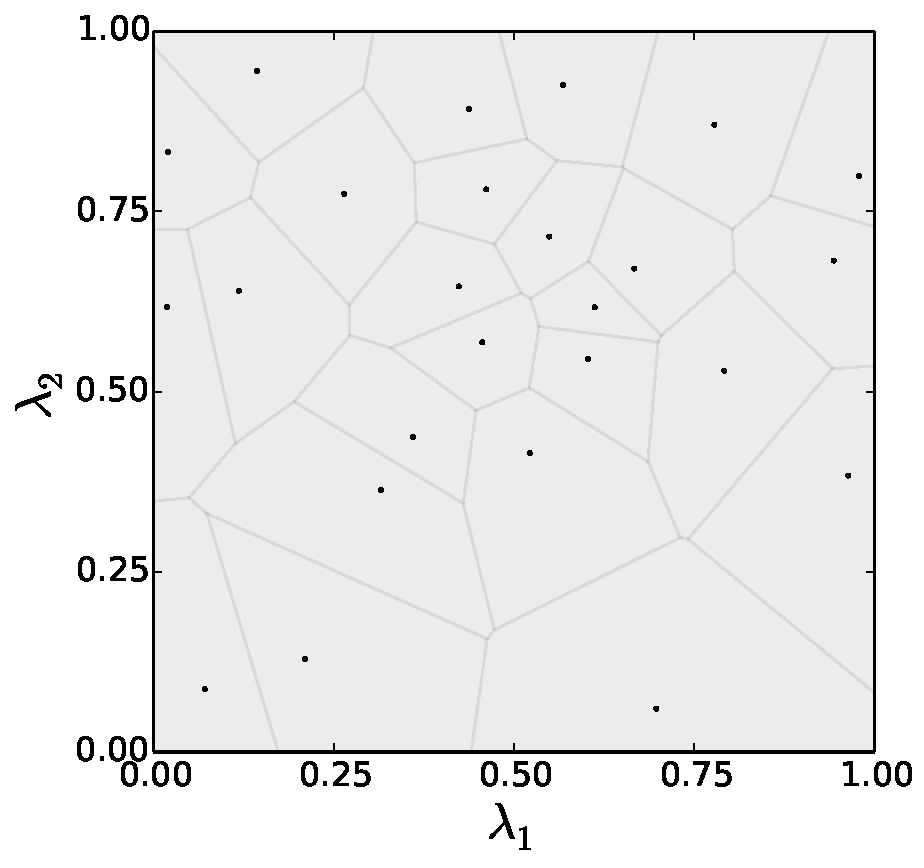
\includegraphics[width=\linewidth]{./images/voronoi_diagram_N25_r0}
	\end{minipage}
	\begin{minipage}{.4875\textwidth}
		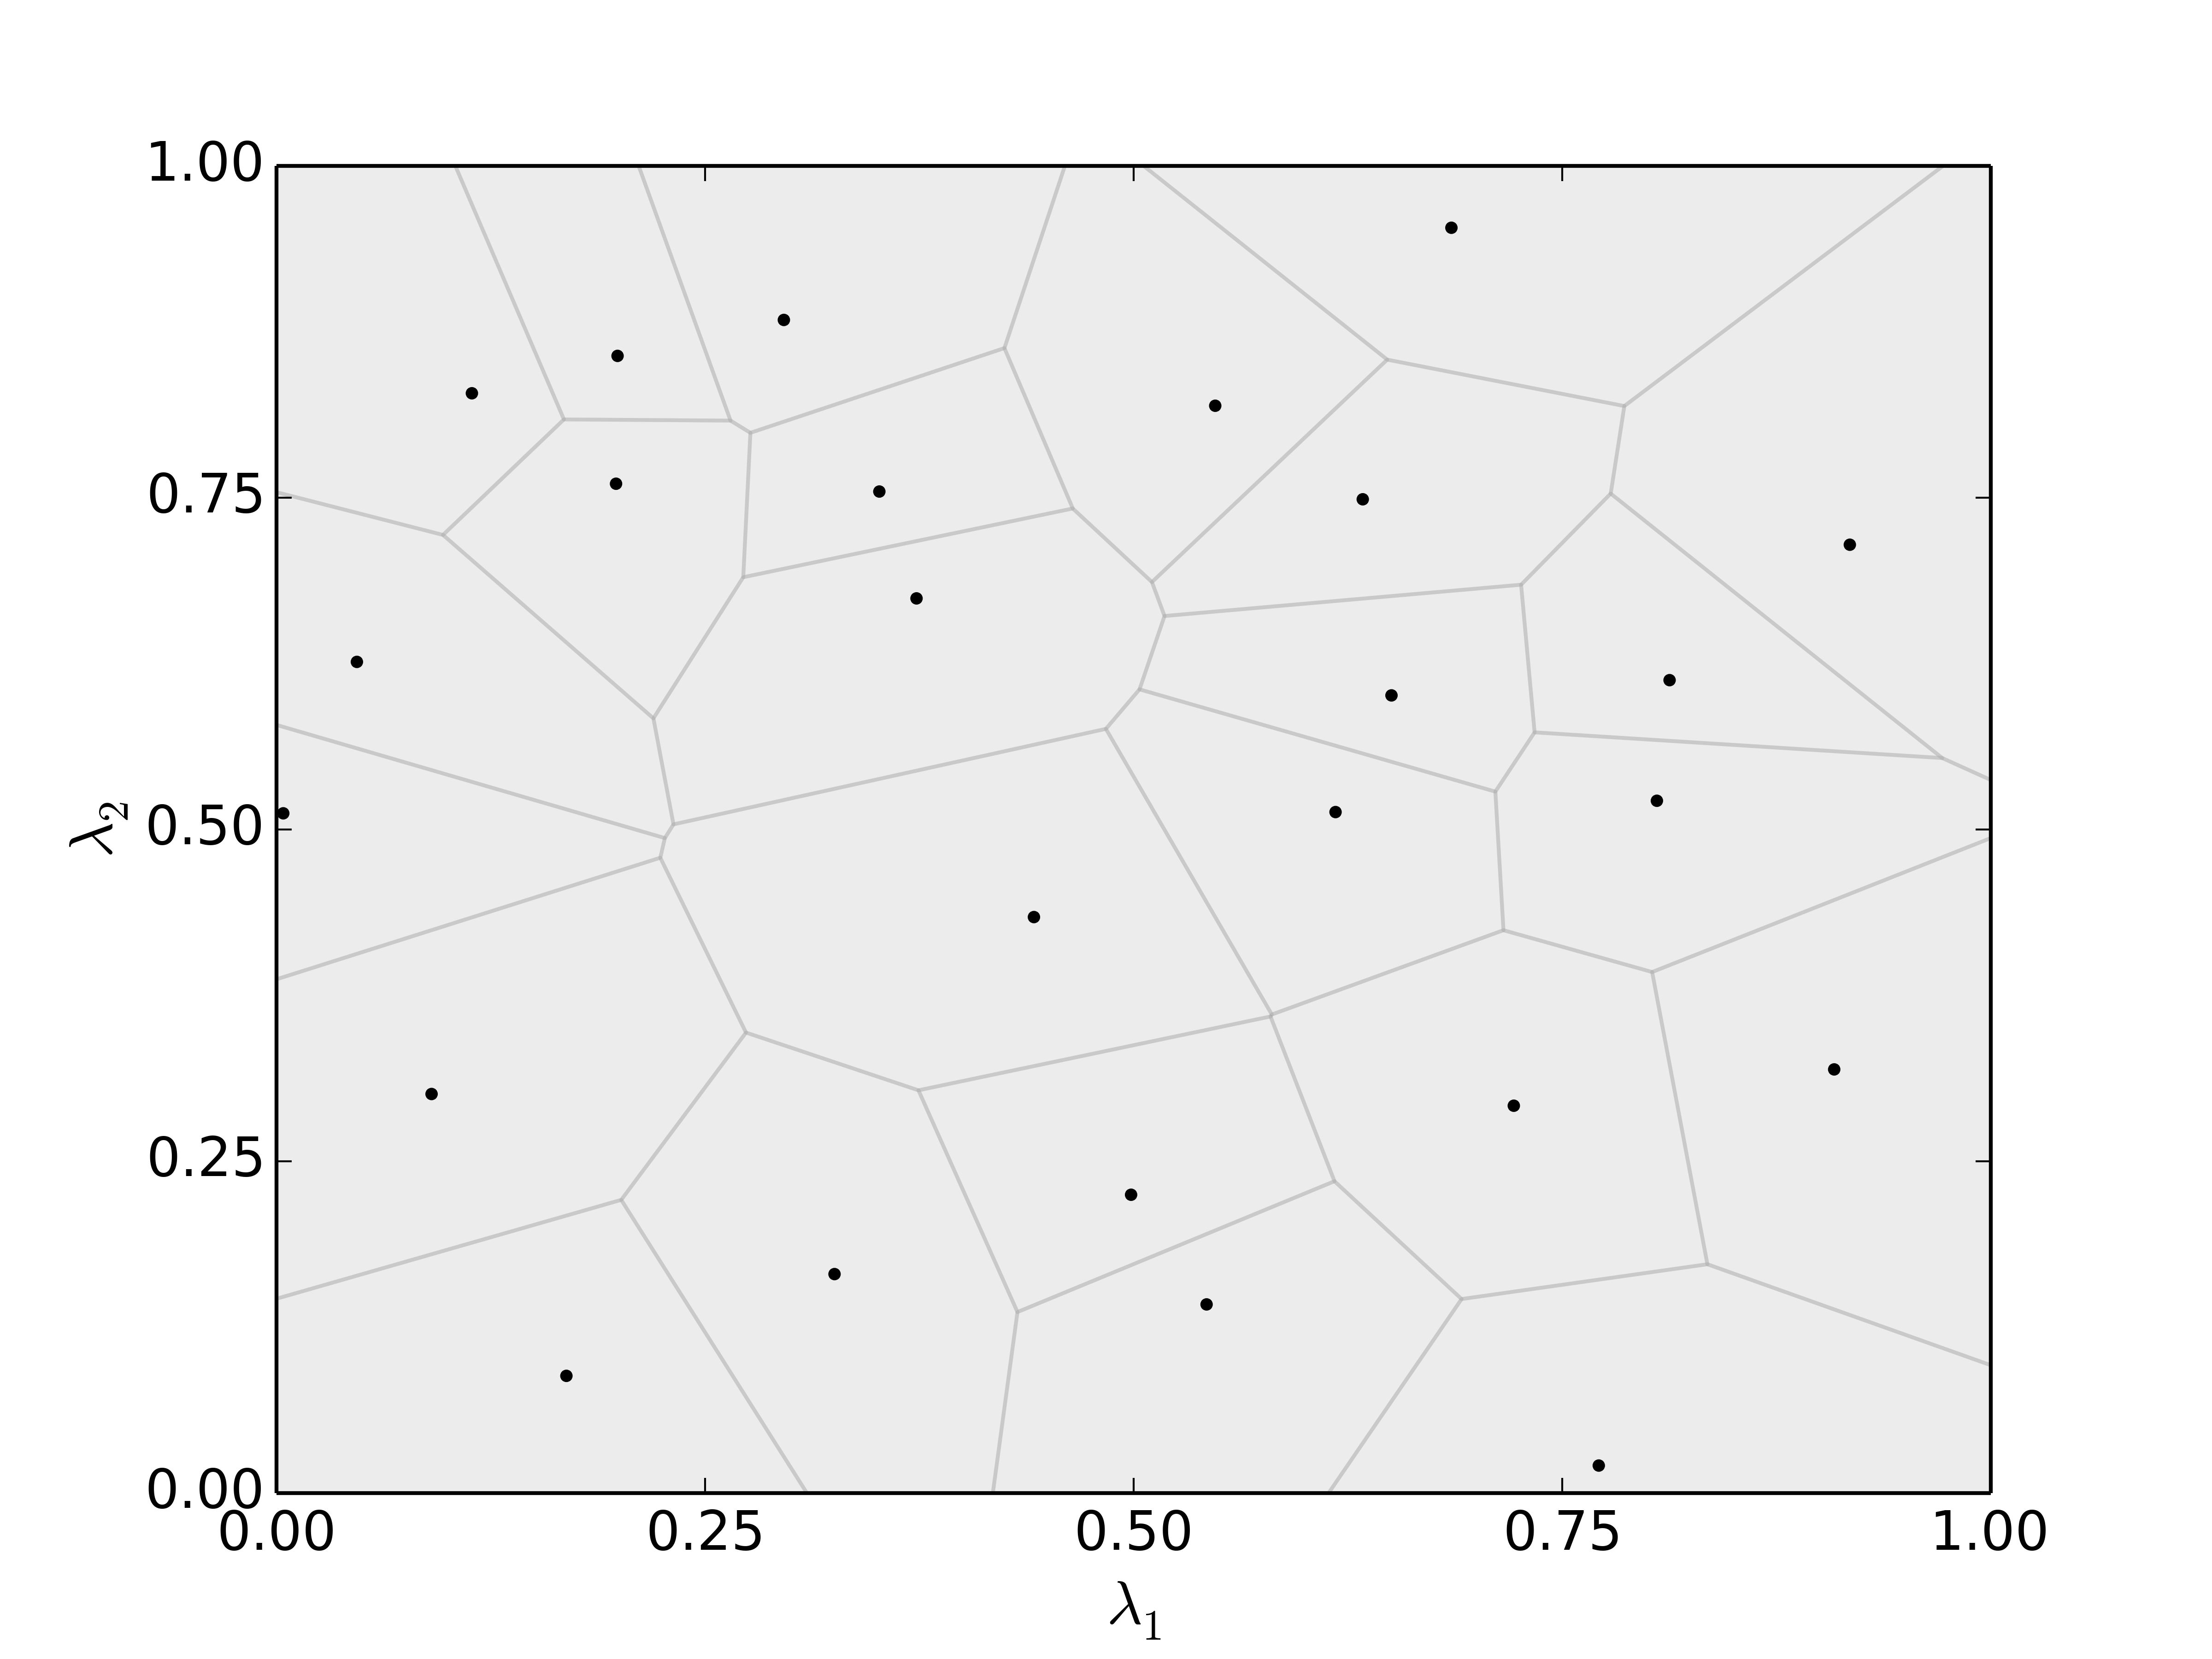
\includegraphics[width=\linewidth]{./images/voronoi_diagram_N25_r10}
	\end{minipage}
\caption{
Two different Voronoi partitions induced by $\nsamps_1 = \nsamps_2 = 25 $ uniform i.i.d.~random samples.
}
\label{fig:voronoi_issues}
\end{figure}


The proof of the following Lemma describes how to ``computationally extend'' {\em any} probability measure defined on a computational algebra to a full $\sa$ $\BB$, which we exploit in Algorithm~\ref{alg:hellinger_disc}.
\begin{lem}
\label{lem:measuresets}
Let $\mu$ be a measure on $(\pspace, \BB_\pspace)$, $\set{\VV^{(j)}}_{j=1}^{\nsamps}$ be a partition of $\pspace$, and $\BB_{\pspace, \nsamps}$ the computational algebra generated by $\set{\VV^{(j)}}_{j=1}^{\nsamps}$.
Assume $\mu (\VV^{(j)}) > 0 \; \forall \; j=1,\hdots, \nsamps$.
Then, there exists a probability measure $\eta$ on $(\pspace, \BB_\pspace)$ such that $\eta(A) = \eta_\nsamps(A) \; \forall \; A\in\BB_{\pspace, \nsamps}$.
\end{lem}
In the proof below, we use $\eta_\nsamps$ and $\mu$ to construct a type of ``discrete'' Radon-Nikodym derivative of $\eta$.
This is motivated by the formal structure of solutions given by Algorithm~\ref{alg:inv_density}.
The proof of Lemma~\ref{lem:measuresets} can be found in Appendix~\ref{app:measuresets}, but the two key equations involved are reproduced here for later reference:

\begin{equation}\label{eq:finiteradon}
f_\nsamps (\param) = \sum_{j=1}^{\nsamps} \frac{\eta_\nsamps (\VV^{(j)}) }{\mu (\VV^{(j)})} \Chi_{\VV^{(j)}} (\param).
\end{equation}

Then, for any $A\in\BB_\pspace$, define

\begin{equation}\label{eq:approxmeasure}
\eta (A) = \int_A f_\nsamps (\param) \, d\mu.
\end{equation}

We note that in practice, $\Chi_{\VV^{(j)}} (\param)$ requires the use of nearest-neighbor computations, but otherwise evaluation of Eq.~\eqref{eq:finiteradon} is straightforward to compute.
With that established, we now present the algorithm used for approximating the distances between pairs of measures (with the computational implementation discussed in \ref{sec:ch03-software}.


\begin{algorithm}
\DontPrintSemicolon
\caption{Hellinger Discretization}
\label{alg:hellinger_disc}
Let $(\pspace, B_{\pspace, \nsamps_1}, \eta_{\nsamps_1} )$ and $(\pspace, B_{\pspace, \nsamps_2}, \eta_{\nsamps_2} )$ be given.\\

Construct $f_{\nsamps_1}$ and $f_{\nsamps_2}$ and corresponding $\eta_1, \eta_2$ using Eq.~\eqref{eq:finiteradon} and Eq.~\eqref{eq:approxmeasure}, respectively.

Use Monte Carlo sampling to approximate
$$ d^2_H(\eta_1, \eta_2) = \int_\pspace \sqrt{f_{\nsamps_1}(\param}) - \sqrt{f_{\nsamps_2}(\param)} \, d\mu $$.
\end{algorithm}

Since we now have a way to extend probability measures defined on $(\pspace, \BB_{\pspace, \nsamps})$ to  probability measure on $(\pspace, \BB_{\pspace})$, we can use simple Monte-Carlo approximation schemes to the Hellinger distance between two probability measures defined on two separate computational algebras.
This is demonstrated in Algorithm~\ref{alg:hellinger_disc}.


%%%%%%%%%%%%%%%%%%%%%%%%%%%%%%%%%%%%%%%%%%%%%%%%%%%%%%%%%%%%%%
\subsection{Overview of Examples}
We establish some fundamental properties of solutions to the SIP under different QoI maps in terms of the skewness of the $Q$'s being compared.
We seek an estimated probability measure $\hat{\PP}_\pspace$ on the parameter space to converge (with respect to the metric $d_\text{TV}$) to some reference measure $\PP_\pspace$ as more samples (i.e., model evaluations), $\nsamps$ are used.
Such a reference measure could be either some known distribution taken as truth, or another approximation deemed to be sufficiently resolved for the given application or computational budget (i.e. higher-fidelity model, mesh, or Monte Carlo sample-size).\footnote{However, we could also choose to interrogate the push-forward measures given by propagating the $\hat{\PP}_\pspace$ and $\PP_\pspace$ forward to a data space by a QoI map and taking the distance on the resulting output space.
This would measure the ability of the maps to reconstruct the output probability measure.}

In Figure~\ref{fig:voronoi_sols}, we illustrate the solution to the problem of comparing measures defined on two different (implicitly-defined) $\sa$s shown in Figure~\ref{fig:voronoi_issues}.
By introducing a third set against which both sample sets of size $\nsamps=50$ are compared, we can leverage theoretical results from Lemma~\ref{lem:measuresets} to compare solutions to the SIP under different QoI maps.

\begin{figure}[ht]
\centering
	\begin{minipage}{.275\textwidth}
		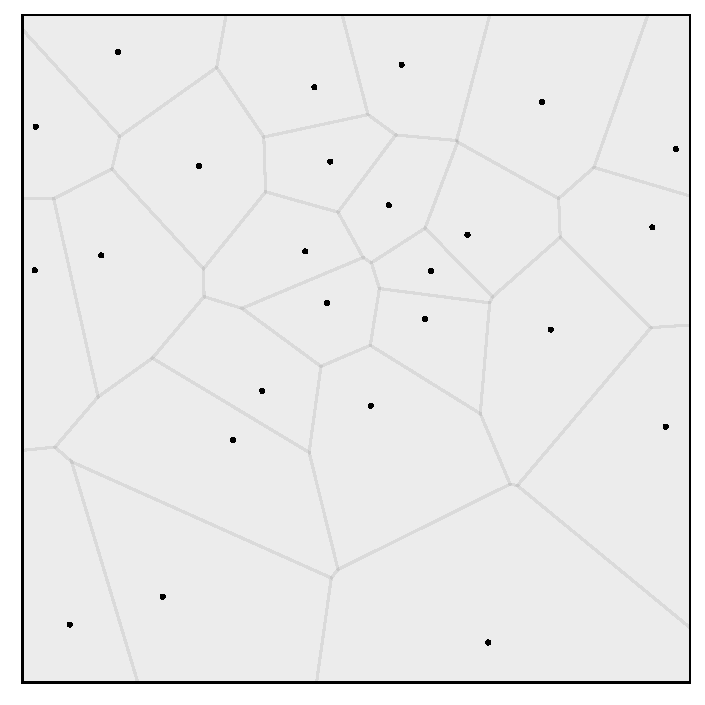
\includegraphics[width=\linewidth]{./images/voronoi_diagrams/voronoi_diagram_N25_r0_no_label}
	\end{minipage}
	\begin{minipage}{.4\textwidth}
		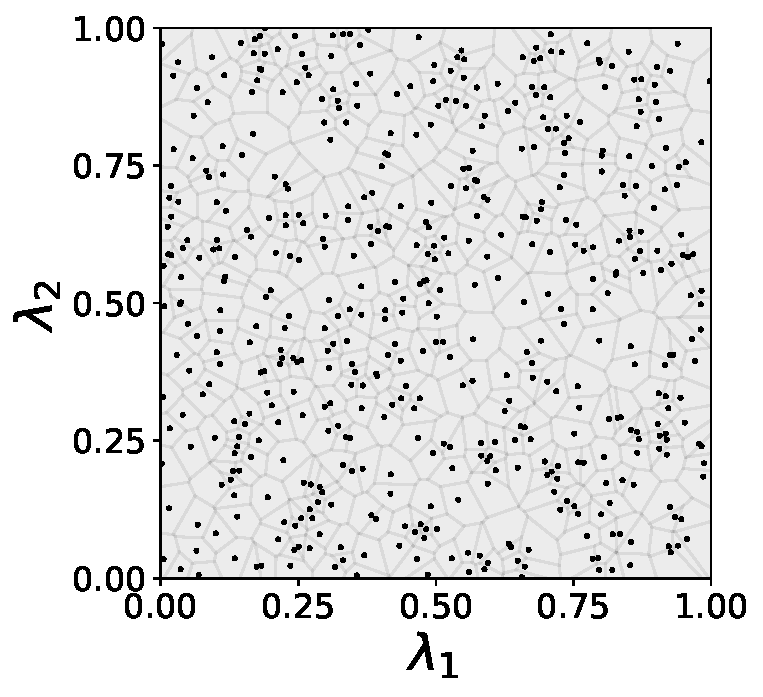
\includegraphics[width=\linewidth]{./images/voronoi_diagrams/voronoi_diagram_N500_r50}
	\end{minipage}
		\begin{minipage}{.275\textwidth}
		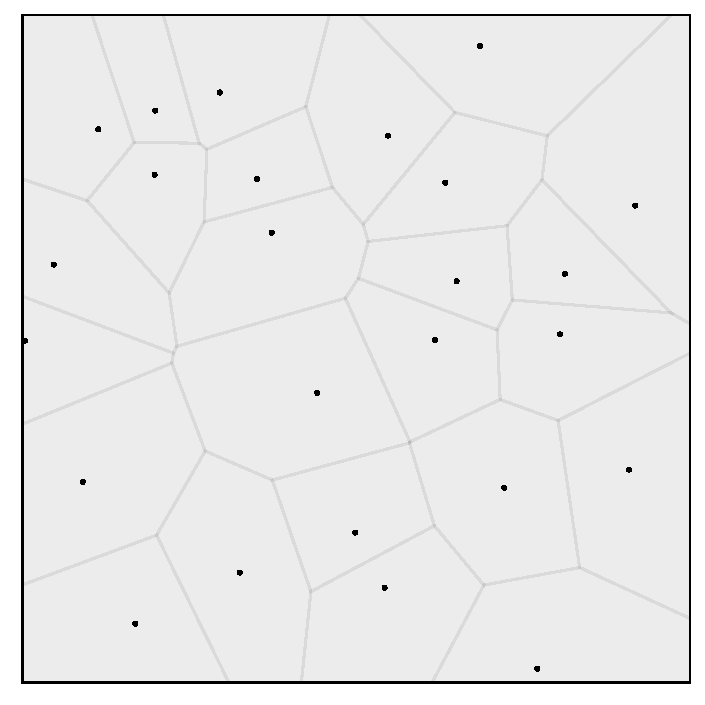
\includegraphics[width=\linewidth]{./images/voronoi_diagrams/voronoi_diagram_N25_r10_no_label}
	\end{minipage}
\caption{
(Left/Right): The two partitions from Figure~\ref{fig:voronoi_issues} will be projected onto a third reference partition (center), in order to compare them on a common $\sa$.
Center: A possibly over-resolved reference sample set, generated using $\nsamps = 500$ uniform i.i.d.~random samples.
}
\label{fig:voronoi_sols}
\end{figure}

To isolate the effect of skewness on the ability to approximate sets with finite sampling, we choose the maps so that they preserve the sizes of sets between $\pspace$ and $\dspace$ under the push-forward measure given in Eq.~\eqref{eq:dataspace_pushforward_measure}.
The sizes of these inverse sets correspond to the average precision of maps $Q$, so we fix the maps to all be equally informative from this perspective; for linear maps, this means they all have the same determinant.

All of our experiments follow the same structure, where $\qspace$ denotes a set of QoI maps under consideration in each example:
\begin{itemize}
\item[[0-a]] Select $\qoi\in\qspace$ and define $\PP_{\dspace_\qoi}$ as a uniform distribution centered on a reference QoI value $Q(\paramref)$ for $\paramref$ taken as the midpoint of $\pspace$.
Note that $\PP_{\dspace_\qoi}$ is exactly discretized with $M=1$ sample, so that
\[
P_{\pspace, 1} = P_\pspace.
\]
\item[[0-b]] Create a regular grid of samples in $\pspace=[0,1]^n$ using $N_{\text{ref},i}$ equispaced points in each dimension.
Set $\bar{N} := \prod N_{\text{ref},i}$.
Since $n$ is small in the numerical examples shown here, we select $N_{\text{ref},i} = 200 \; \forall \; i$ in each example.
\item[[0-c]] Use Algorithm~\ref{alg:inv_density} to construct a reference solution $\PP_{\pspace,\bar{N}}\approx \PP_\pspace$.
\item[[1]] Generate $\set{S_k^{(n)}}_{n=1}^{50}$ sets of uniform i.i.d.~random samples where $N_k = 25, 50, 100, 200, \hdots, 6400$, and $n$ represents the number of repeated trials of a sample size $N_k$.
%, constructing $\set{\set{\VVV_k^{(j)}}_{k=1}^{50}}_{j=1}^{N}$ so that when we compute Total Variation distances on the approximate measures defined on each $\set{\VVV_k^{(j)}}{j=1}{N}$, we can reduce the variance in our expected Total Variation distance values for each instance of $N$. Note that we experimented with using more trials and found the variance in expected Total Variation distances was sufficiently low with as few as twenty trials for the maps under consideration herein.
%\item[[3]] For every trial $T$ and $N$ value (including $\bar{N}$), the reference parameter $\lambda = (\lambda_1, \lambda_2) = (0.5, 0.5)$ is mapped by $Q$ to $\dspace_\qoi = Q(\pspace)$.
%\item[3] A uniform distribution with support $[Q(\lambda_1) - 0.05, Q(\lambda_1) + 0.05] \times [Q(\lambda_2) - 0.05, Q(\lambda_2) + 0.05]$ is defined on $\dspace_\qoi$, representing equal uncertainty in each component of our measured functional values.
\item[[2]] Solve the SIPs using Algorithm~\ref{alg:inv_density} to construct $\set{\PP_{\pspace,M,N}^{(n)}}_{n=1}^{50}$.
\item[[3]] Use $1E5$ i.i.d.~random samples to estimate $\set{d_H^2( \PP_{\pspace,M,N}^{(n)}, \PP_{\pspace,\bar{N}})}_{n=1}^{50}$.
\item[[4]] Average over all trials $n$ for each $N$ to estimate the {\em expected} Total Variation distance for $N$ samples and analyze convergence to $\PP_{\pspace,\bar{N}}$.
\item[[5]] Repeat steps [0-a]--[4] for each $\qoi\in\qspace$ under consideration.
\end{itemize}

\FloatBarrier

\subsection{Rotational Invariance}\label{ex:rotation}
This example shows that if $\qoiA$ is defined by a rotation of $\qoiB$, then the accuracy and convergence rates of $\PP^{(a)}_{\pspace, \ndiscs, \nsamps}$ are identical to $\PP^{(b)}_{\pspace, \ndiscs, \nsamps}$.
We expect this to be true since skewness is rotationally invariant, as we summarize in the following Proposition.
\begin{prop}
The quantity $S_\qoi(\param)$ is invariant under rotations performed on $\qoi$ for any $\param$. \\
\label{prop:rot_invariance}
\end{prop}
\begin{proof}
If we apply a rotation $\qoi$, then the Jacobians $J_{\qoi, \param}$ are also subject to the same rotation at each $\param$.
Since rotations are unitary operators, the norms given in Eq.~\eqref{eq:skewness} used to define skewness are unaffected.
\end{proof}

\begin{figure}
\begin{minipage}{.5\textwidth}
\begin{table}[H]
\begin{tabular}{ c | c | c | c }
\nsamps & $\qoiA$ & $\qoiB$ & $\qoiC$\\ \hline \hline
$200$ & $2.18E-01$ & $1.97E-01$ & $2.19E-01$\\ \hline

$400$ & $1.60E-01$ & $1.70E-01$ & $1.51E-01$\\ \hline

$800$ & $1.09E-01$ & $1.14E-01$ & $1.09E-01$\\ \hline

$1600$ & $7.43E-02$ & $7.76E-02$ & $7.53E-02$\\ \hline

$3200$ & $5.51E-02$ & $5.53E-02$ & $5.31E-02$\\ \hline

$6400$ & $4.19E-02$ & $4.09E-02$ & $4.19E-02$\\ \hline
\end{tabular}
\end{table}
\end{minipage}
\begin{minipage}{.45\textwidth}
		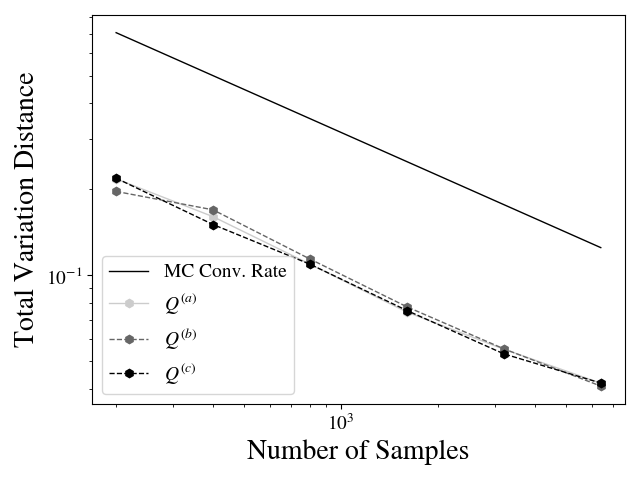
\includegraphics[width=\linewidth]{./images/Plot-orth-reg_BigN_40000_reg_M_1_rand_I_100000.png}
\end{minipage}
\caption{The results of $d^2_\text{TV}(\PP_{\pspace, \ndiscs, \nsamps}, \PP_{\pspace, \bar{\nsamps}})$ for three maps generated by random rotations of orthogonal linear maps.}
\label{fig:M1orth}
\end{figure}

To demonstrate this Lemma numerically, we define the space of QoI maps $\qspace = \set{ \qoiA , \qoiB, \qoiC }$, where all three are linear maps with the same local skewness $S_\qoi (\param) = 1 \; \forall \param \in \pspace$.
The map $\qoiA$ is the identity and the other two, $\qoiB$ and $\qoiC$ are rotations of $\qoiA$ by randomly chosen angles.
Following the algorithmic outline above, we perform a convergence study to $\PP_{\pspace,\bar{\nsamps}}$ with results summarized in Figure~\ref{fig:M1orth}.
The convergence rates and expected errors in the SIPs associated with each of these maps are virtually indistinguishable.
In light of Proposition~\ref{prop:rot_invariance} and these numerical results, we conclude that the accuracy of the numerical solution to the SIP is invariant under rotations to the QoI map.

\FloatBarrier

%%%% 2D Skewness Example %%%%%% 
\subsection{Impact of Skewness on Accuracy}\label{ex:skewness}
In this example, we demonstrate the key point of this study: the magnitude of skewness between QoI impacts accuracy by orders of magnitude, and thus in optimizing the choice of a QoI map, it is in our interest to pursue the minimization of skewness. 
This is especially true in problems where the number of random samples we are permitted to use is constrained by the computational cost of model evaluations.

%Thus, any map can be thought of as a piecewise-defined linear map, and the results we present in this example, while applying to all of $\pspace$ in these cases, can be applied solely to the support of each local linear approximation.
%Capturing the geometry of sets (improving accuracy) on each of these subdomains thus guarantees a desired result on the entirety of the domain. 

To illustrate this point, we first define the linear maps 
\begin{equation}\label{eq:qmap2}
\qspace_S := \left \lbrace Q^{(s)} =  \mat{cc}{1 & 0 \\ \sqrt{s^2 - 1}& 1 } \right \rbrace_{s\in S},
\end{equation}
for $S=\set{1,2,4}$ because they allow us to control the global skewness (since it is equal to local skewness in a linear map) while preserving the measures of sets between $\pspace$ and $\dspace$. 
More specifically, the support of the solution to the SIP associated with each QoI map has equal $\mu_\pspace$-measure, which isolates the impact of accuracy solely to the skewness of the QoI map.
We show what the component row vectors of these maps in Figure~\ref{fig: skewmapvecs} and note the skewness is determined by the ratio of the magnitude of the black line to its projection onto the vertical axis (and each of these projects directly on to the unit vector).  
The skewness of these maps is given by the index $s$, so $Q^{(1)}$ is $1$, the skewness of $Q^{(2)}$ is $2$, and $S_{Q^{(4)}} = 4$.

The maps chosen for this example are expository ones that provide valuable insight despite their simplicity. 
For example, when solving many physics-based problems, local linear approximations are often used to simplify model evaluation and guide optimization procedures.


\begin{figure}[h]
	\begin{minipage}{.3\textwidth}
		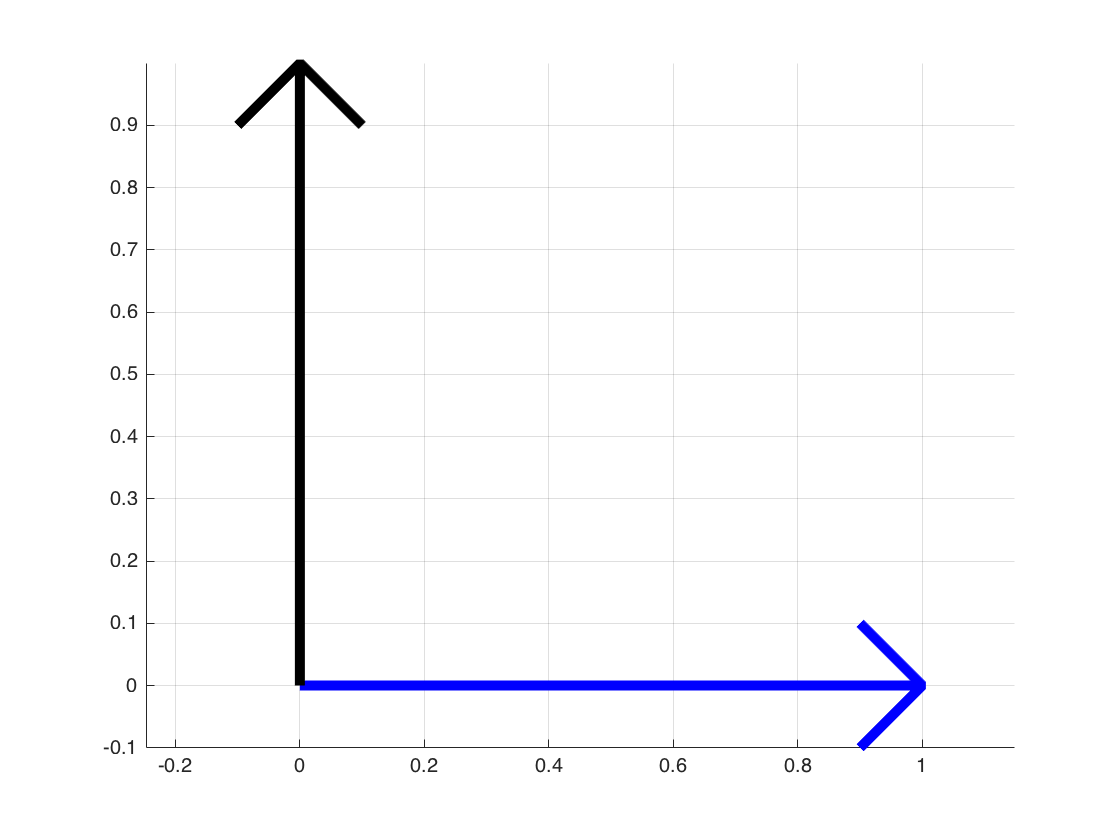
\includegraphics[width=\linewidth]{./images/vector_a.png}
	\end{minipage}
	\begin{minipage}{.3\textwidth}
		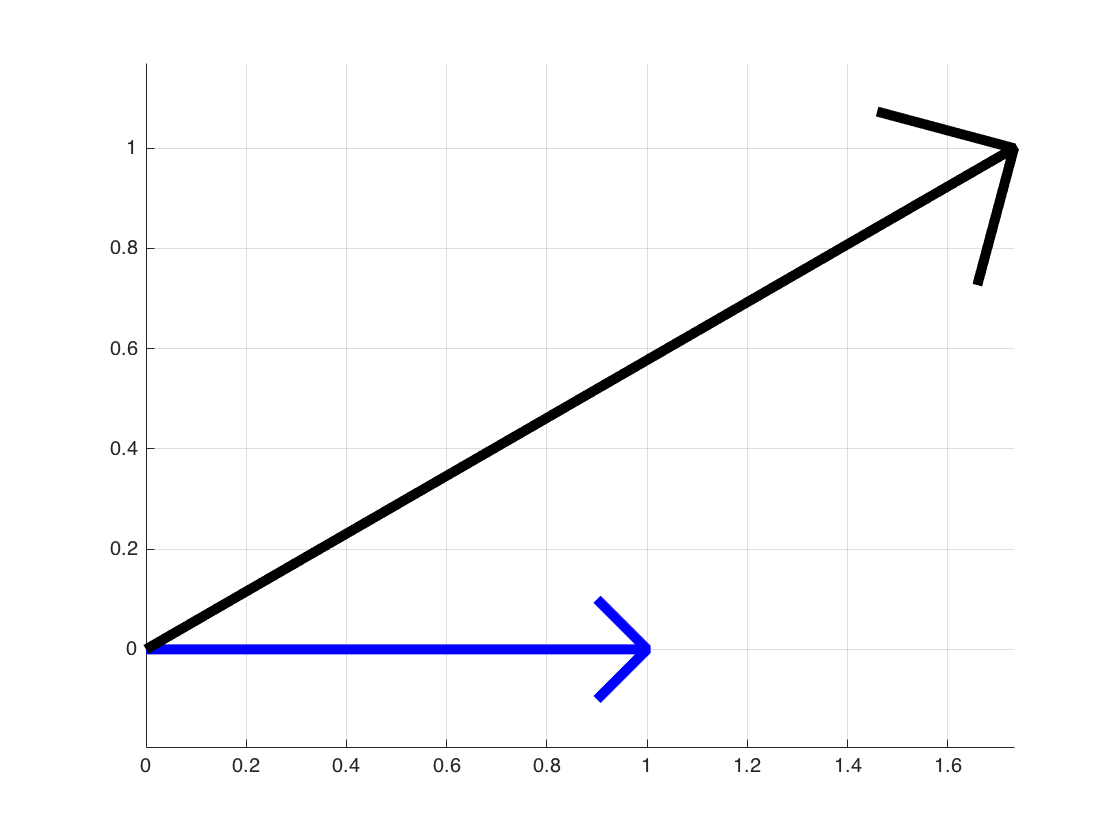
\includegraphics[width=\linewidth]{./images/vector_b.png}
	\end{minipage}
	\begin{minipage}{.3\textwidth}
		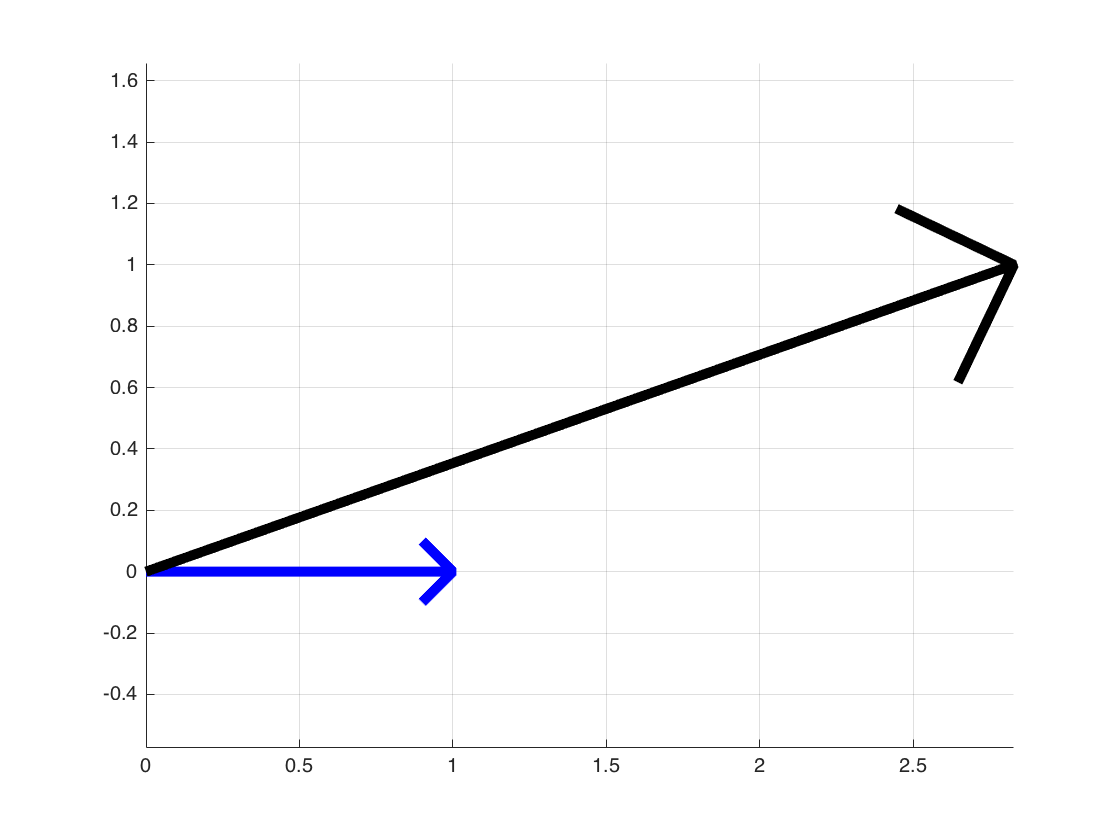
\includegraphics[width=\linewidth]{./images/vector_c.png}
	\end{minipage}
\caption{(Left to right):  The component row-vectors of $Q^{(1)}$, $Q^{(2)}$, and $Q^{(4)}$. Our linear maps take $\RR^2$ to $\RR^2$ and can be visualized graphically as the component row-vectors of the matrices representing the transformation. The first row is highlighted in blue. The skewness is then simply equal to the reciprocal of the inverse sine of the angle between these vectors. }
\label{fig: skewmapvecs}
\end{figure}


\begin{figure}
\begin{minipage}{.5\textwidth}
\begin{table}[H]
\begin{tabular}{ c | c | c | c }
N & $Q^{(1)}$ & $Q^{(2)}$ & $Q^{(4)}$\\ \hline \hline
$200$ & $1.35E-01$ & $2.03E-01$ & $3.12E-01$\\ \hline 
 
$400$ & $9.96E-02$ & $1.47E-01$ & $2.15E-01$\\ \hline 
 
$800$ & $7.19E-02$ & $1.04E-01$ & $1.53E-01$\\ \hline 
 
$1600$ & $5.27E-02$ & $7.49E-02$ & $1.10E-01$\\ \hline 
 
$3200$ & $3.70E-02$ & $5.25E-02$ & $7.52E-02$\\ \hline 
 
$6400$ & $2.76E-02$ & $3.86E-02$ & $5.54E-02$\\ \hline 
\end{tabular}
\end{table}
\end{minipage}
\begin{minipage}{.45\textwidth}
		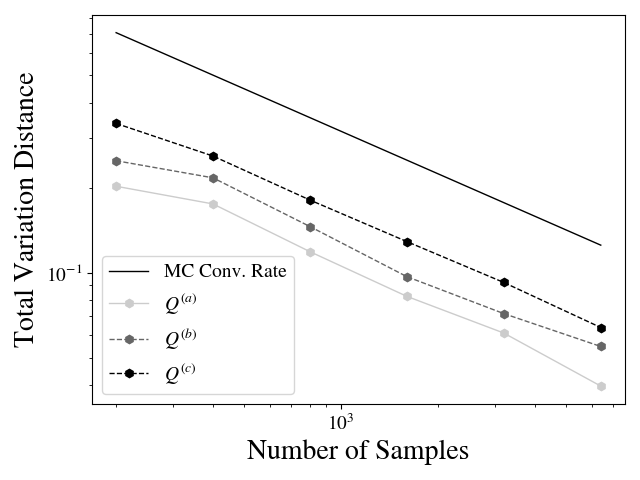
\includegraphics[width=\linewidth]{./images/Plot-reg_BigN_40000_reg_M_1_rand_I_100000}
\end{minipage}
\caption{The results of $d^2_H(\PP_{\pspace, M, N}, \PP_{\pspace,\bar{N}})$.}
\label{fig:M1_2d}
\end{figure}

We see in Figure~\ref{fig:M1_2d} that skewness has a very direct impact on the number of samples required to achieve a particular value for the Hellinger distance. 
We can see that the measure induced by $Q^{(1)}$ requires fewer than half the number of samples to be as accurately resolved as $Q^{(2)}$ does. 
The effect is even more pronounced when compared against $Q^{(4)}$.
It appears that if the ratio of skewness between two maps is 2, then the more-skewed map will require at least twice as many random samples to approximate the set on a a well-resolved discretization with the same error tolerance.

This provides a strong motivation for minimizing skewness and reinforces the results from \cite{BPW_2015}, where it was demonstrated that a similar relationship existed in the number of samples required to remove error in inverse set approximations quantified by the $\mu_\pspace$-measure of the {\em symmetric difference} of the inverse sets.




%%%% 3D Skewness Example %%%%%%

\subsection{Dependence on Dimension}\label{ex:3dmap}
To further illustrate that relationship between skewness and accuracy holds as we move towards higher dimensions, we extend the numerical investigation to a three--dimensional parameter space.
Generally, we have fewer QoI than number of uncertain model parameters, so we assume that the potential QoI maps are defined by the $2\times 3$ matrices
\begin{equation}\label{eq:qmap3}
\qspace_S := \left \lbrace \qoi^{(s)} =  \mat{ccc}{1 & 0 & 0\\ \sqrt{s^2 - 1}& 1 & 0} \right \rbrace_{s\in S}.
\end{equation}
Here, as in the previous example, the index $s$ indicates the magnitude of skewness.
Furthermore, the results of Example~\ref{ex:rotation} justify the restriction of the maps to this form since any linear map of skewness $s$ is simply a rotation of maps of this form.

%Now, the generalized contours for inverses of maps from $\RR^3 \to \RR^2$ will be isomorphic to 2\--dimensional contour events in that the inverse sets will be columns in 3\-space orthogonal to the aforemntioned plane.
%
%IMAGE DEMONSTRATING THIS WOULD HELP.
%We define
%
%which is just the map from \eqref{eq:qmap2} appended with zeros in the third column.
%We make this choice solely for convience and are justified in doing so owing to Proposition~\ref{prop:rot_invariance} and the fact of generalized contours of maps from $\RR^3 \to \RR^2$ being parallel columns.
%The rotational invariance naturally extends to the third dimension.

%We note that $\bar{N}$ is much higher since we kept the convention of 200 grid cells per dimension in our reference.
%However, we kept the same number of random samples $N$, so we should expect higher errors due to the overresolved regular grid.
%Fortunately, we find that the results still generalize.
%We present the case where $M=1$:

\begin{figure}[h]
\begin{table}[H]
\begin{tabular}{ c | c | c | c }
\nsamps & $\qoiA$ & $\qoiB$ & $\qoiC$\\ \hline \hline
$200$ & $3.33E-01$ & $4.56E-01$ & $6.10E-01$\\ \hline

$400$ & $2.78E-01$ & $3.51E-01$ & $4.97E-01$\\ \hline

$800$ & $2.19E-01$ & $2.95E-01$ & $4.10E-01$\\ \hline

$1600$ & $1.72E-01$ & $2.37E-01$ & $3.35E-01$\\ \hline

$3200$ & $1.36E-01$ & $1.89E-01$ & $2.64E-01$\\ \hline

$6400$ & $1.09E-01$ & $1.47E-01$ & $2.09E-01$\\ \hline
\end{tabular}
\end{table}

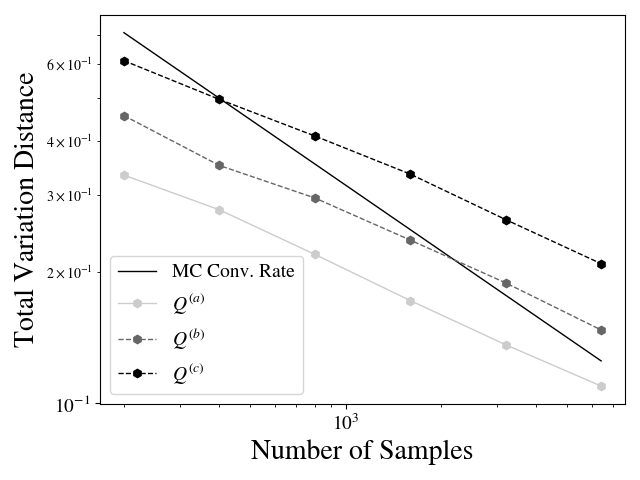
\includegraphics[width=0.45\linewidth]{./images/Plot-reg_BigN_8000000_reg_M_1_rand_I_100000.png}

\caption{The results of $d^2_\text{TV}(\PP_{\pspace, \ndiscs, \nsamps}, \PP_{\pspace, \ndiscs, \bar{\nsamps}})$ for $\ndiscs = 1, \bar{\nsamps} = 8,000,000$, with $a, b, c = 1, 2, 4$ in three dimensions.}
\label{fig:M1_3d}
\end{figure}
\FloatBarrier
In Figure~\ref{fig:M1_3d}, it appears that the effect of skewness is even more pronounced in higher dimensions, and that the number of samples required to achieve similar levels of accuracy between two maps with a ratio of skewness 2 is now quadrupled.
The analysis of \cite{BGE+15} suggested a dependence of accuracy related to the skewness raised to a power related to the dimension of the data space.

%%%%%%%%%%%%%%%%%%%%%%%%%%%%%%%%%%%%%%%%%%%%%%%%%%%%%%%%%%%%%%

\
\section{Accuracy of Sample-Based Inversion}\label{sec:ch03-sample}

How does the new approach compare? What role does the KDE play in the error?
Focus on linear problems. One or two examples (perhaps use that skew-map with 1 and 2 and 4).

%%%% Sample-Based Skewness Example %%%%%%

\subsection{A Sample-Based Solution}\label{eq:sampleskew}

Here we solve the problems in Examples~\ref{ex:skewness} and~\ref{ex:3dmap}, except in the framework of the Sample-Based Inversion outlined in \ref{sec:ch02-sample}.
Effect of Skewness appears to be mitigated.
\vfill{10in}

%%%%%%%%%%%%%%%%%%%%%%%%%%%%%%%%%%%%%%%%%%%%%%%%%%%%%%%%%%%%%%

\
\section{Software Contributions}\label{sec:ch03-software}

Talk about the BET module that computes metrics.
Discuss testing, show sample of usage (disconnected from skewness, high-level).


\
\section{Numerical Results and Analysis}\label{sec:ch03-approx}

\subsection{Convergence with Repeated Observations}
2D but with repeated data, show how the measures converge. Should be identical to the differences in the observed densities.

\subsection{Nonlinear Example}
Maybe heatrod here?

%%%%%%%%%%%%%%

Pick an ODE problem and show how the results look like (assimilating as many data points as inputs, if using time-series model).

Our goal in this section is to provide a set of examples that demonstrate these two approaches, their ``solutions.''
Exponential Decay, uncertain initial condition and rate. Fix two measurement times. No OED discussion.

Show visualization of solution on voronoi-mesh vs. 2D density.

This is going to set up the stage nicely.
What if we had more measurements to incorporate? Discuss how the distributions we imposed as our observed were kind of a little disingenuous since they were based on single measurements. Well, rather, they represent the answer to a different question.
